\documentclass[a4paper,titlepage]{article}
\title{CT Projekt: Raycasting Game Engine II (Huskyrock)}
\author{Christian Korn}
\date{14.01.2022 - 04.06.2022}

\usepackage[utf8]{inputenc}
\usepackage[ngerman]{babel}
\usepackage[pdftex]{graphicx}
\usepackage{amssymb}

\tolerance=1
\emergencystretch=\maxdimen
\hyphenpenalty=10000
\hbadness=10000

\begin{document}
    
    \maketitle
    \tableofcontents
    
    %%%%%%%%%%%%%%%%%%%%%%%%%%%%%%%%%%%%%%%%%%%%%%%%%%%%%%%%%%%%%%%%%%%%%%%%%%%%
    
    \newpage
    
    \section{Ziele}
    
    \subsection{Muss-Ziele}
    
    \subsubsection*{Hundefels}
    
    Das neue Projekt muss die Kernfunktionalität des Vorgängerprojektes enthalten:
    
    \begin{itemize}
        \item Anzeigen eines 2D Levels in 2,5D per Raycasting \checkmark
        \item Bewegungsfreiheit im Level \checkmark
        \item Anzeige von Entities im Level \checkmark
        \item Kollisionserkennung \checkmark
    \end{itemize}
    
    \subsubsection*{Neues}
    
    Natürlich soll das neue Projekt auch eigene Features und Technologien enthalten, die es vom Alten unterscheiden:
    
    \begin{itemize}
        \item Wand-Texturen \checkmark
        \item Sprites für Entities \checkmark
        \item KI für Entities \checkmark
    \end{itemize}
    
    Das neue Projekt wird in der Programmiersprache Rust geschrieben,
    anstatt eines objektorientierten Designs wird ein Entity component system benutzt.
    
    \subsection{Kann-Ziele}
    
    \subsubsection*{Hundefels}
    
    Einige Features des Vorgängerprojektes werden als Kann-Ziele klassifiziert, da sie nicht für die Funktionalität des Projektes absolut notwendig sind.
    
    \begin{itemize}
        \item Laden von Leveln aus externen Dateien (durch neue features komplizierter)
        \item Command-Line Argumente (Funktionalität größtenteils überflüssig oder besser als Konfigurationsdatei zu lösen)
    \end{itemize}
    
    \subsubsection*{Andere}
    
    \begin{itemize}
        \item Visuelle Effekte (view-bobbing, etc.)
        \item Schießen
        \item Kartenansicht
        \item WebAssembly
        \item unterschiedliche Sprites für verschiedene Drehwinkel
    \end{itemize}
    
    %%%%%%%%%%%%%%%%%%%%%%%%%%%%%%%%%%%%%%%%%%%%%%%%%%%%%%%%%%%%%%%%%%%%%%%%%%%%
    
    \newpage
    
    \section{Verwendete Technologien}
    
    \subsection{Rust}
    
    Rust ist eine Multiparadigmen-Systemprogrammiersprache mit einem Fokus auf Performance und Sicherheit. Dies wird erreicht, indem anstatt eines Garbage Collectors oder händischem Memory managements ein sogenannter Borrow Checker verwendet wird, der Lifetimes und Scope von Variablen überprüft und Regeln für Referenzen durchsetzt.
    
    \subsection{Entity component system}
    
    Entity component system (kurz ECS) ist ein Softwarearchitekturmuster, welches vor allem in der Spieleentwicklung genutzt wird.\\
    Im Gegensatz zu objektorientierten Programmen werden im ECS Daten und Funktionalität nicht gruppiert, sondern getrennt in sogenannte ``Components'' (Daten) und ``Systems'' (Funktionalität).
    Zentral im ECS sind die ``Entities'': Objekte, die Components enthalten, auf welche Systems angewandt werden.\\
    Systems können spezifizieren, welche Components für sie notwendig sind und werden nur auf die Entities angewandt, die alle benötigten Components enthalten.\\
    Zum Beispiel wird in diesem Projekt mit einem Component definiert, ob eine Entity der Spieler ist, und deshalb eine Kamera enthalten sollte, mit einem anderen ob die Entity mit einer KI ausgestattet ist. Entities ohne diese beiden Components sind stationär oder bewegen sich gleichförmig ohne steuerung (abhängig davon, ob sie die Bewegungs-Component enthält).
    
    \subsection{A*}
    
    Der A*-Algorithmus ist ein Suchalgorithmus, der einen Optimalen Pfad zwischen zwei Punkten findet. Durch eine Kostenfunktion und eine Heuristik wird dabei die Laufzeit des Algorithmus optimiert.
    
    \subsection{Raycasting}
    
    Raycasting ist eine Methode mit welcher die Entfernung zu Geometrie effizient berechnet werden kann. Es wurde in frühen 3D Spielen genutzt um einen 3D-Effekt in einer 2D Welt vorzutäuschen.
    
    \subsection{Tools}
    
    \begin{itemize}
        \item IDE: Intellij IDEA mit Rust Extension
        \item Grafiksystem: SDL2
        \item Dokumentation: Overleaf online \LaTeX Editor, \\
        \verb|https://www.overleaf.com|
        \item Pixelart: Pixilart, \\
        \verb|https://www.pixilart.com/|
    \end{itemize}
    
    %%%%%%%%%%%%%%%%%%%%%%%%%%%%%%%%%%%%%%%%%%%%%%%%%%%%%%%%%%%%%%%%%%%%%%%%%%%%
    
    \newpage
    
    \section{Mathematische Funktionsweise}
    
    Alle Berechnungen außer dem A* Algorithmus werden 60 mal pro Sekunde ausgeführt, A* wird pro Entity ein mal pro Sekunde berechnet.
    
    \subsection{Bewegung}
    
    Die aktuelle Position, Rotation, maximale Geschwindigkeit, relative Geschwindigkeit und Rotationsgeschwindigkeit werden, soweit anwendbar, in den Components \verb|Position|, \verb|Rotation|, \verb|VelocityMultiplier| und \verb|VelocityRelative| gespeichert, das Input des Spielers in \verb|PlayerInput| und die Kontrollarten werden durch \verb|UserControlled| und \verb|HasAI| markiert. \\
    
    Die neue Position und Rotation jeder Entity werden berechnet mit:
    
    $$x_{t+1} = x_t + (-vr_x*\cos{r} - vr_y*\sin{r})$$
    $$y_{t+1} = y_t + (-vr_y*\cos{r} + vr_x*\sin{x})$$
    
    Zur Kollisionserkennung werden 4 Punkte um die Entity überprüft, ob sie ein Block sind, wenn ja wird die Position der Entity angepasst.
    
    \subsection{Rendering}
    
    \subsubsection*{Raycasting}
    
    Von der Entity ausgehend werden Strahlen in Paaren ausgesendet:
    
    Der horizontale Strahl überprüft bei vertikalen Linien, der vertikale Strahl bei horizontalen Linien.
    Mit dem Unterschied der Richtung funktionieren beide insgesamt gleich, die Erklärung konzentriert sich daher auf den horizontalen Strahl.\\
    
    Zuerst wird der x-Wert des Strahls $x_{ray}$ auf die nächste Linie gesetzt, danach der y-Wert $y_{ray}$ mit folgender Formel bestimmt: 
    
    $$y_{ray} = x_{entity}-x_{ray}*\frac{-1}{\tan(\alpha_{ray})}+y_{entity}$$
    
    Nun wird der Strahl wiederholt um 1 in $x$-Richtung und um
    
    $$-block\_size * \frac{-1}{\tan(\alpha_{ray})}$$
    
    in $y$-Richtung verschoben. Nach jedem Verschieben wird überprüft, um es sich beim neuen Block um eine Wand handelt, wenn ja wird abgebrochen und die zurückgelegte Entfernung, sowie die x- und y-Koordinaten des Strahls zurückgegeben.\\
    
    Von den zwei so berechneten Werten wird nun der kürzere Strahl ausgewählt, auf der Karte gezeichnet und als vertikale Linie  der Länge
    
    $$v\_offset = \frac{1}{dist + 0,001} * v\_multiplier $$
    
    im Viewport angezeigt ($dist$ ist die Länge des Strahls, die zwei festen Werte verhindern, dass durch 0 geteilt wird und erhöhen den Wert auf eine sichtbare Länge).
    
    \subsubsection*{Beispiel}
    
    \setlength{\unitlength}{1cm}
    Horizontaler Check, vertikaler Strahl:\\\\
    \begin{picture}(5,4)
        % Gitternetz
        \multiput(0,0)(1,0){6}{\line(0,1){4}}
        \linethickness{0.4mm}
        \multiput(0,0)(0,1){5}{\line(1,0){5}}
        \thinlines
        % Wand
        \multiput(0,0)(0.1,0){50}{\line(0,1){1}}
        % Spieler und Sichtlinie
        \put(1,3){\circle*{0.3}}
        \thicklines
        \put(1,3){\vector(4,-3){2.7}}
        % Kreuzpunkte
        \linethickness{0.6mm}
        \put(2.35,1.75){\line(0,1){0.5}}
        \put(2.1,2){\line(1,0){0.5}}
        \put(3.68,0.75){\line(0,1){0.5}}
        \put(3.43,1){\line(1,0){0.5}}
    \end{picture}\\\\
    Vertikaler Check, horizontaler Strahl:\\\\
    \begin{picture}(5,4)
        % Gitternetz
        \linethickness{0.4mm}
        \multiput(0,0)(1,0){6}{\line(0,1){4}}
        \thinlines
        \multiput(0,0)(0,1){5}{\line(1,0){5}}
        % Wand
        \multiput(0,0)(0.1,0){50}{\line(0,1){1}}
        % Spieler und Sichtlinie
        \put(1,3){\circle*{0.3}}
        \thicklines
        \put(1,3){\vector(4,-3){3}}
        % Kreuzpunkte
        \linethickness{0.6mm}
        \put(2,2){\line(0,1){0.5}}
        \put(1.75,2.25){\line(1,0){0.5}}
        \put(3,1.25){\line(0,1){0.5}}
        \put(2.75,1.5){\line(1,0){0.5}}
        \put(4,0.5){\line(0,1){0.5}}
        \put(3.75,0.75){\line(1,0){0.5}}
    \end{picture}
    
    \subsubsection*{Entities}
    
    Die x-Position einer Entity im Viewport wird mit folgender Formel berechnet:
    
    $$\frac{r_{player} + atan2(dy, dx)}{fov} * fensterbreite$$
    
    Einige Korrekturen werden dabei noch vorgenommen, um die Position der Entity auf dem Bildschirm nicht umherspringen zu lassen.\\
    
    Zuerst werden die Strahlen hinter der Entity angezeigt, dann die Entity selbst und zuletzt die Strahlen vor der Entity.
    
    \newpage
    
    \subsection{KI}
    
    \subsubsection*{Steuerung}
    
    Jede Entity mit den notwendigen Components überprüft jeden Frame, ob der Spieler hinter einer Wand ist. Ist dass der Fall, wird der nächste Punkt auf dem per A* berechneten Pfad als Ziel gewählt, ansonsten der Spieler. Zeigt die Entity auf das gewählte Ziel, geht sie mit voller Geschwindigkeit vorwärts, ansonsten dreht sie sich in Richtung Ziel und geht mit verringerter Geschwindigkeit vorwärts.
    
    \subsubsection*{A*}
    
    Einmal Pro Sekunde wird der A* Algorithmus von jeder Entity mit den nötigen Components ausgeführt. \\
    
    Jedem Knoten werden im Laufe des Algorithmus 4 Werte zugeordnet: $f$, $g$, $h$ und der Vorgängerknoten. $g$ ist die bisherige Kostenfunktion auf dem weg zum Knoten, $h$ ist die Heuristik, mit der die Kosten zum Ziel geschätzt werden und $f$ ist die Summe aus $g$ und $h$. \\
    Es werden zuerst zwei Listen angelegt: die OpenList und die ClosedList. Der OpenList wird nun der Startknoten mit einem $f$ von 0 hinzugefügt. \\
    solange die OpenList nicht leer ist passiert folgendes: \\
    Es wird der Knoten $q$ mit dem niedrigsten $f$ von der OpenList entfernt, seine Nachfolgeknoten generiert und für jeden dieser Knoten nun überprüft, ob er der Zielknoten ist, in welchem Fall die Suche beendet wird. \\
    Ansonsten $f$ für den Knoten generiert. Wenn der Knoten mit niedrigerem $f$ in der OpenList oder ClosedList ist wird er übersprungen. Ansonsten wird der Knoten der OpenList hinzugefügt. Zuletzt wird $q$ der ClosedList hinzugefügt. \\
    
    Nachdem der A* Algorithmus selbst beendet ist wird vom Zielknoten ausgehend die Route generiert, indem sich entlang der Vorgängerknoten durch die ClosedList gehangelt wird und die entstandene liste umgedreht wird.
    
    
    %%%%%%%%%%%%%%%%%%%%%%%%%%%%%%%%%%%%%%%%%%%%%%%%%%%%%%%%%%%%%%%%%%%%%%%%%%%%
    
    \newpage
    
    \section{Programmaufbau}
    
    \begin{itemize}
        \item \verb|main.rs| ist der Programmeinstiegspunkt und enthält den Großteil des    Setups, sowie die Gameloop.
        \item \verb|init.rs| enthält code zum Erstellen von Entities für den Spieler, Gegner und Gegenstände.
        \item \verb|components.rs| enthält die Components für das ECS
        \item \verb|ai.rs| enthält das KI-System und die A* Implementation
        \item \verb|input.rs| ist für die Verarbeitung von Playerinput zu Bewegungsvektoren verantwortlich
        \item \verb|physics.rs| führt die Bewegungsbefehle des Spielers oder der KI aus
        \item \verb|render.rs| stellt entities und rays dar
        \item \verb|rays.rs| berechnet das Raycasting
    \end{itemize}
    
    %%%%%%%%%%%%%%%%%%%%%%%%%%%%%%%%%%%%%%%%%%%%%%%%%%%%%%%%%%%%%%%%%%%%%%%%%%%%
    
    \newpage
    
    \section{Steuerung}
    
    \subsection{Bewegung}
    
    \subsubsection*{Translation (Laufen)}
    \begin{itemize}
        \item Vorwärts: `W'
        \item Links: `A'
        \item Rückwärts: `S'
        \item Rechts: `D'
    \end{itemize}
    
    \subsubsection*{Rotation}
    \begin{itemize}
        \item Links: linke Pfeiltaste ($\leftarrow$)
        \item Rechts: rechte Pfeiltaste ($\rightarrow$)
    \end{itemize}
    
    \subsection{UI}
    
    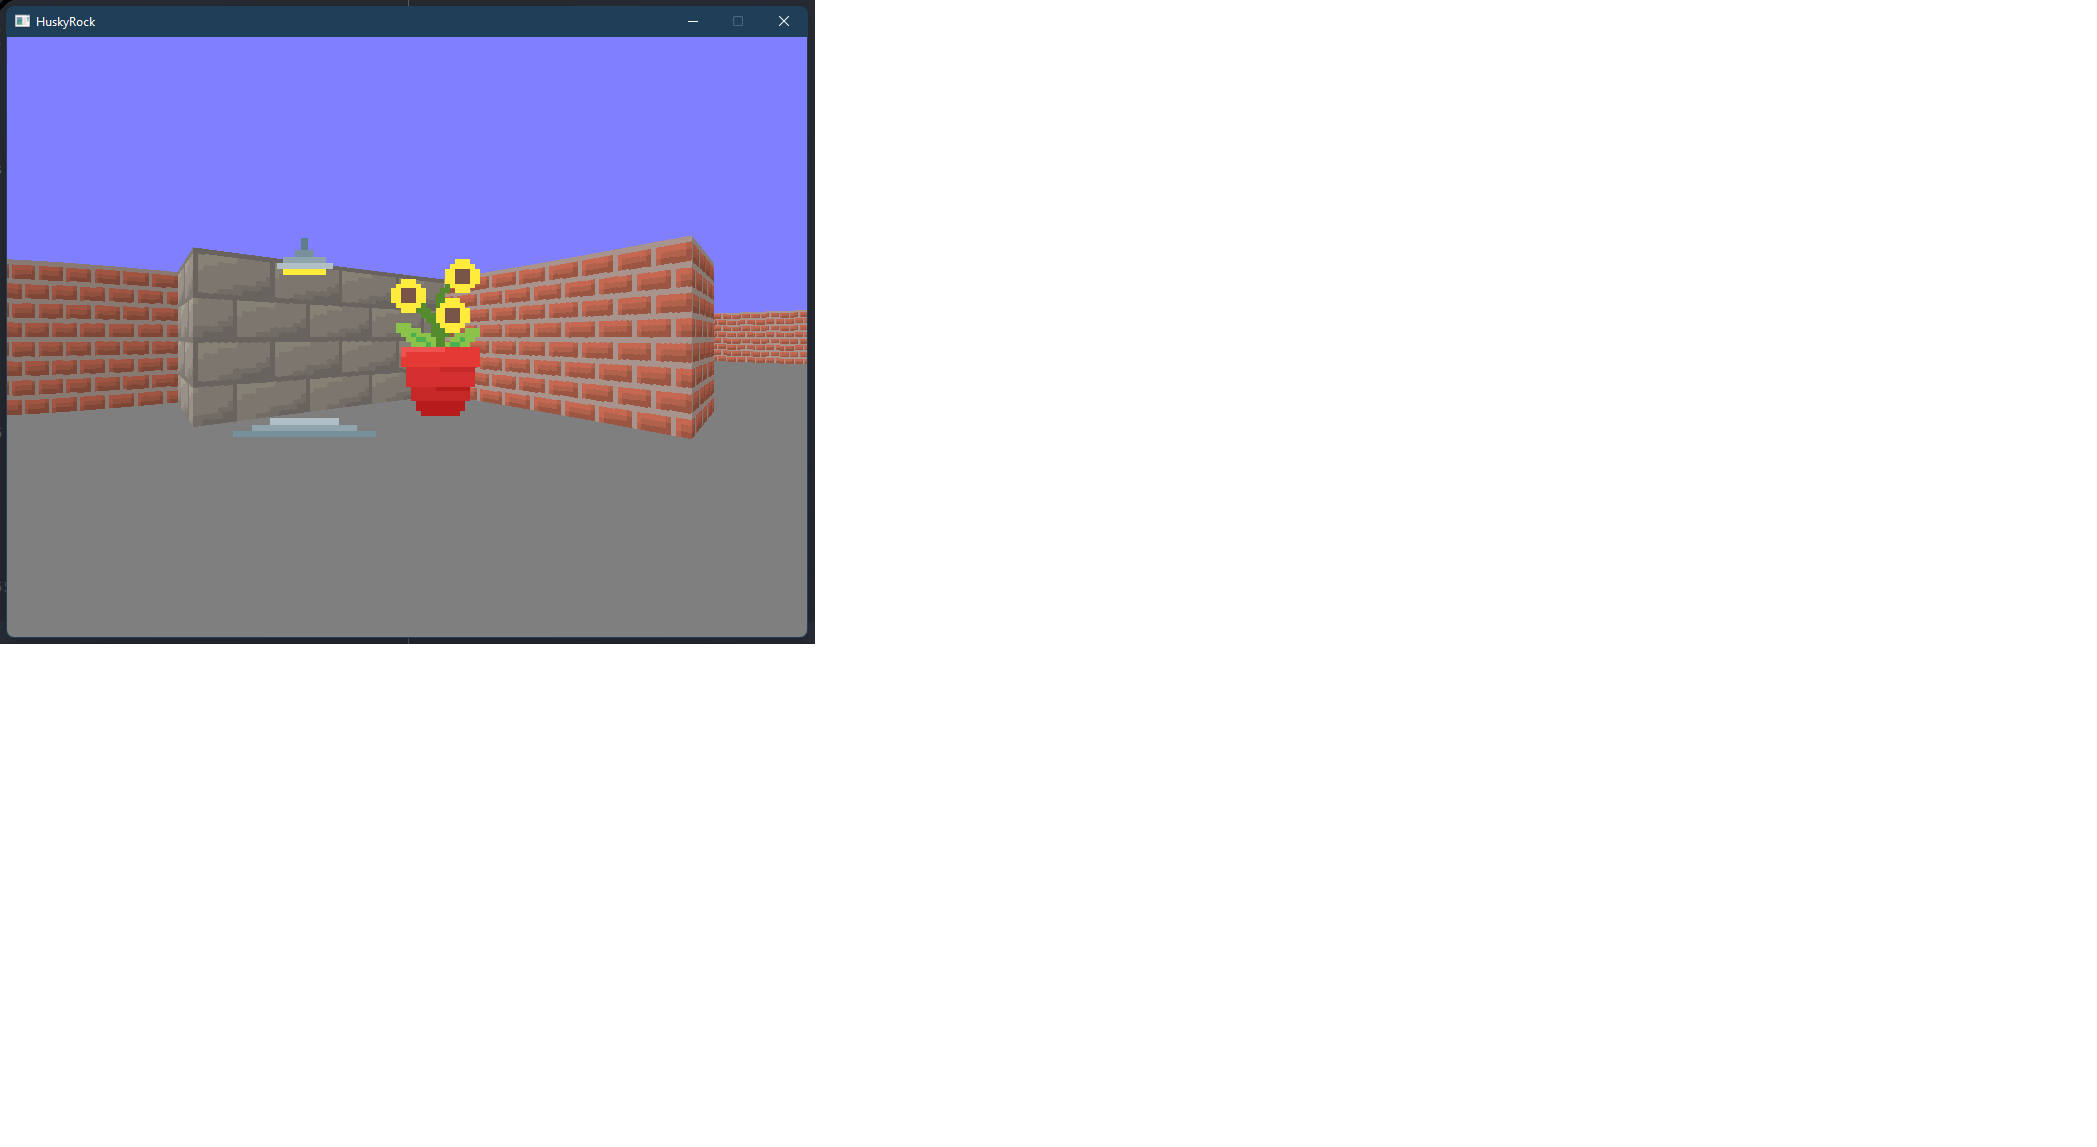
\includegraphics[scale=0.57]{demo_screenshot.png}
    
    Zu sehen sind:
    \begin{itemize}
        \item Verschiedene Wandtexturen (Lehmziegel, Steinziegel), bei der Kartenerstellung frei wählbar
        \item Verschiedene Texturen für verschiedene Seiten, automatisch (abhängig von der Seite)
        \item Zwei Entities mit verschiedenen Texturen, bei der Kartenerstellung frei wählbar
    \end{itemize}
    
    %%%%%%%%%%%%%%%%%%%%%%%%%%%%%%%%%%%%%%%%%%%%%%%%%%%%%%%%%%%%%%%%%%%%%%%%%%%%
    
    \newpage
    
    \section{Quellen}
    
    Das GIT-repository findet sich unter \\
    \verb|https://github.com/MacAphon/husky_rock|
    
    \begin{itemize}
        \item Viel Code wurde direkt vom Vorgängerprojekt zu Rust übersetzt und wiederverwendet. \\
        \verb|https://github.com/MacAphon/hundefels2d|
        
        \item Steve Klabnik \& Carol Nichols: ``The Rust Programming Language'' \\
        \verb|https://doc.rust-lang.org/stable/book/|
        
        \item ``Rust by Example'' \\
        \verb|https://doc.rust-lang.org/rust-by-example/|
        
        \item ``Rust Coockbook'' \\
        \verb|https://rust-lang-nursery.github.io/rust-cookbook/|
        
        \item ``Learn Game Development in Rust'' \\
        \verb|https://sunjay.dev/learn-game-dev| \\
        \verb|https://github.com/sunjay/rust-simple-game-dev-tutorial/|
        
        \item 3DSage: ``Make Your Own Raycaster Part 1'' \\ 
        \verb|https://youtu.be/gYRrGTC7GtA|\\ 
        Quellcode verfügbar unter \\
        \verb|https://github.com/3DSage/OpenGL-Raycaster\_v1|
        
        \item A* Search Algorithm - GeeksforGeeks \\
        \verb|https://www.geeksforgeeks.org/a-search-algorithm/|
    \end{itemize}
    
\end{document}